%20 min preso!
\documentclass[xcolor=table,english]{beamer}
\usepackage{beamerthemesplit}
\usepackage{wrapfig}
\usetheme{SPbGU}
\usepackage{pdfpages}
\usepackage{amsmath}
\usepackage{mathtools}
\usepackage{cmap}
\usepackage{subcaption}
\usepackage[utf8]{inputenc}
\usepackage[T1, T2A]{fontenc}
\usepackage[]{babel}
\usepackage{indentfirst}
\usepackage{amsmath}
\usepackage{tikz}
\usepackage{multirow}
\usepackage[noend]{algpseudocode}
\usepackage{algorithm}
\usepackage{algorithmicx}
\usepackage{fancyvrb}
\usetikzlibrary{calc}
\usetikzlibrary{shapes,arrows}
\usetikzlibrary{arrows,automata}
\usetikzlibrary{positioning}
\usetikzlibrary{fit}

\usepackage{kbordermatrix} % include package @ document preamble
\renewcommand{\kbldelim}{(} % change default array delimiters to parentheses
\renewcommand{\kbrdelim}{)}

\newcommand\mca{\multicolumn{1}{c}{\cellcolor{red}\textbf{\{a\}}}}
\newcommand\mcb{\multicolumn{1}{c}{\cellcolor{red}\textbf{\{b\}}}}

\usepackage{tabularx}
\newcolumntype{Y}{>{\raggedleft\arraybackslash}X}

\renewcommand{\thealgorithm}{}

\newtheorem{mytheorem}{Theorem}
\renewcommand{\thealgorithm}{}

\newcommand{\tikzmark}[1]{\tikz[overlay,remember picture] \node (#1) {};}
\def\Put(#1,#2)#3{\leavevmode\makebox(0,0){\put(#1,#2){#3}}}

\newcommand{\ltz}{$< 1$}

\tikzset{
    state/.style={
           rectangle,
           rounded corners,
           draw=black, very thick,
           minimum height=2em,
           inner sep=2pt,
           text centered,
           },
}

\beamertemplatenavigationsymbolsempty

\title[Kronecker CFPQ GPGPU]{Реализация алгоритма поиска путей с КС ограничениями в графовых БД через произведение Кронекера на платформе Nvidia CUDA}
% \subtitle[YaccConstructor]{Parsing techniques for graph analysis}
% То, что в квадратных скобках, отображается в левом нижнем углу.
\institute[СПбГУ]{
JetBrains Research, Лаборатория языковых инструментов  \\
Санкт-Петербургский Государственный университет
}

% То, что в квадратных скобках, отображается в левом нижнем углу (прикольно).
\author[Егор Орачев]{\textbf{Егор Орачев}}
\date{19 декабря 2020}


\begin{document}
{
\begin{frame}[fragile]
  \begin{table}
  \centering
  \begin{tabularx}{\linewidth}{YcX}
    
\includegraphics[height=1.5cm]{pictures/jetbrainsResearch.pdf} \hfill
    & \begin{minipage}[t]{0.3\textwidth}\center \vspace{-1cm} Миниконференция
      \end{minipage}
    & \hfill 
\includegraphics[height=1.5cm]{pictures/SPbGU_Logo.png}
  \end{tabularx}
  \end{table}
  \titlepage
\end{frame}
}

\begin{frame}[fragile] \frametitle{Введение}
    \begin{minipage}[m]{0.5\linewidth}
        \begin{figure}
            \centering
            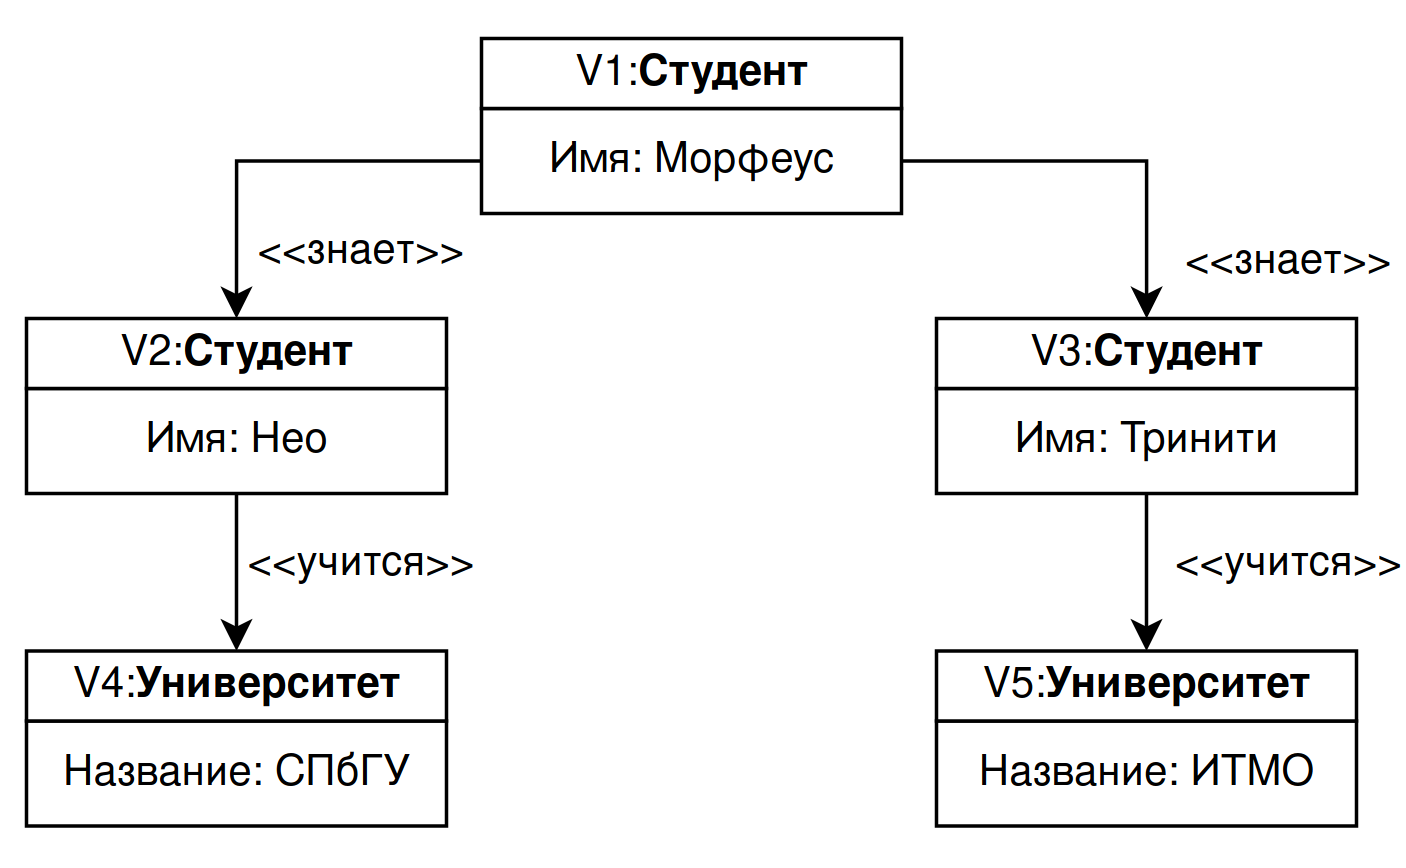
\includegraphics[width=\textwidth]{figures/db_example.png}
            \caption{Пример графовой БД}
            \label{fig:architecture}
        \end{figure}
    \end{minipage}\hfill
    \begin{minipage}[m]{0.5\linewidth}
        \begin{itemize}
            \item Графовая модель данных
            \item Графовые базы данных
            \item Запросы к графовым базам данных
            \item Использование КС грамматик как формализма для формирования запроса
        \end{itemize}
    \end{minipage}
\end{frame}

\begin{frame}[fragile] \frametitle{Запросы с КС ограничениями}
    \begin{minipage}[m]{0.45\linewidth}
        \begin{figure}
            \centering
            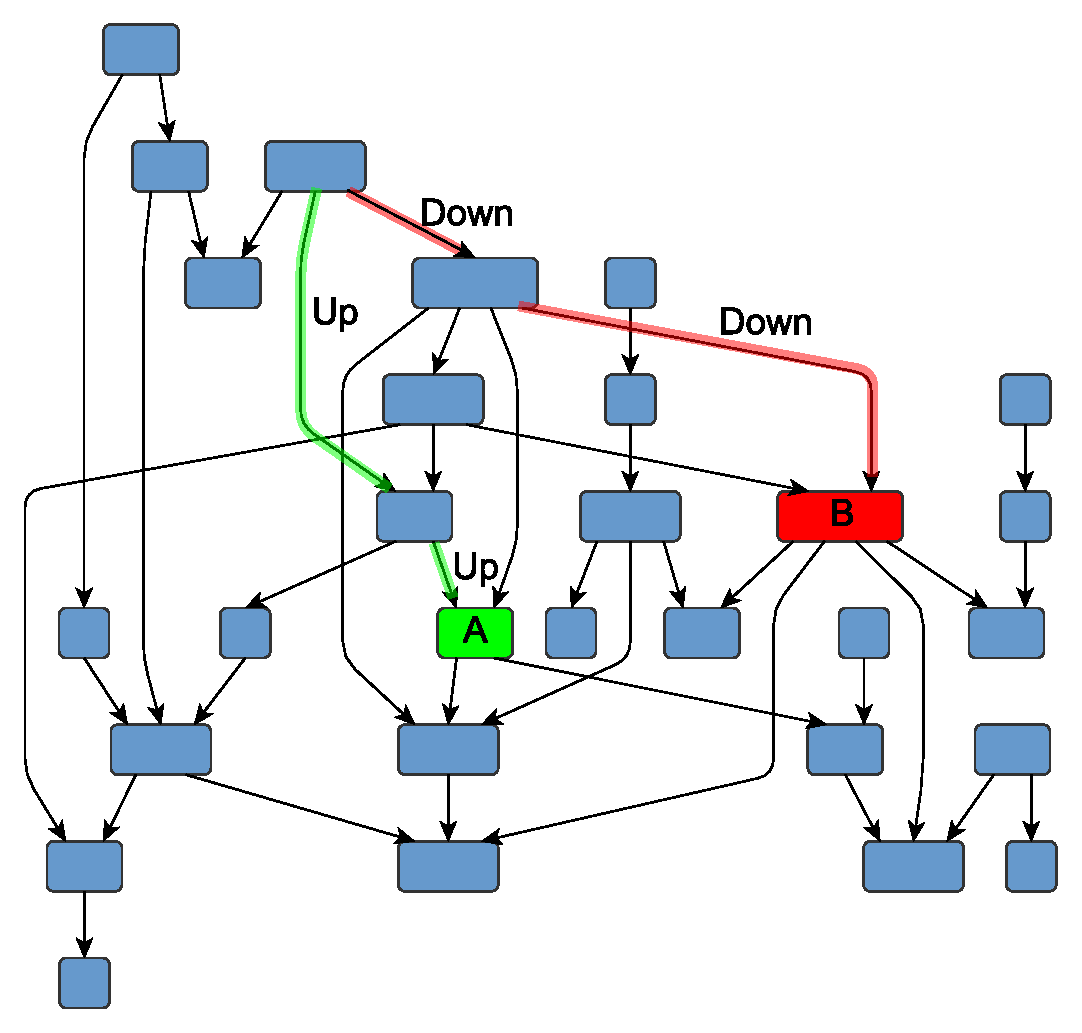
\includegraphics[width=\textwidth]{pictures/hierarchical.pdf}
            \caption{Пример графа}
        \end{figure}
    \end{minipage}\hfill
    \begin{minipage}[m]{0.5\linewidth}
        Навигация в графе:
        \begin{itemize}
            \item Находятся ли вершины A и B на одном уровне иерархии?
            \item Существует ли путь вида $\textbf{Up}^n \, \textbf{Down}^n$?
            \item Найти все такие пути $\textbf{Up}^n \, \textbf{Down}^n$, которые начинаются в вершине~А
        \end{itemize}
  \end{minipage}
\end{frame}

\begin{frame}[fragile] \frametitle{Семантика запроса}
    \begin{itemize}
        \item Ориентированный граф с меткаи $\mathcal{G} = \langle V, E, L \rangle$
        \item $\omega(\pi) = \omega(v_0 \xrightarrow{l_0} v_1 \xrightarrow{l_1} \cdots \xrightarrow{l_{n-2}} v_{n-1} \xrightarrow{l_{n-1}} v_n) = l_0 l_1 \cdots l_{n-1}$
        \item КС Грамматика $G = \langle \Sigma, N, P, S \rangle$
        \item Язык $L(G) = \{ w~|~S \rightarrow^*_G w \}$
        \item Семантика достижимости: $R = \{ (u, v) ~|~ \exists u \pi v: \omega(\pi) \in L \}$
        \item Семантика всех путей: $\Pi = \{ u \pi v ~|~ \omega(\pi) \in L \}$
    \end{itemize}
\end{frame}

\begin{frame}[fragile] \frametitle{Пример запроса}
    \begin{itemize}
        \item Пример запроса:\\MATCH $(u) \rightarrow [:\verb|знает|] \rightarrow () \rightarrow [:\verb|учится|] \rightarrow (v)$\\RETURN $u, v$
        \item Семантика достижимости:\\ $\{ (V1, V4), (V1, V5) \}$
        \item Семантика всех путей:\\ $\{ (V1 \overset{\textit{знает}}{\rightarrow} V2 \overset{\textit{учится}}{\rightarrow} V4), (V1 \overset{\textit{знает}}{\rightarrow} V3 \overset{\textit{учится}}{\rightarrow} V5) \}$
    \end{itemize}
\end{frame}

\begin{frame}[fragile] \frametitle{Существующие алгоритмы для вычисления КС запросов}
    \begin{itemize}
        \item Алгоритмы, основанные на различных техниках парсинга \\ (CYK, LL, LR, etc.)
		\item Алгоритм Рустама Азимова на основе операций линейной алгебры\\(реализация на CPU, на GPU)
		\item \textbf{Алгоритм на основе произведения Кронекера}\\(реализация на CPU, на GPU?)
    \end{itemize}
\end{frame}

\begin{frame}[fragile] \frametitle{GPGPU} 
    \begin{minipage}[m]{0.45\linewidth}
        \begin{figure}
            \centering
            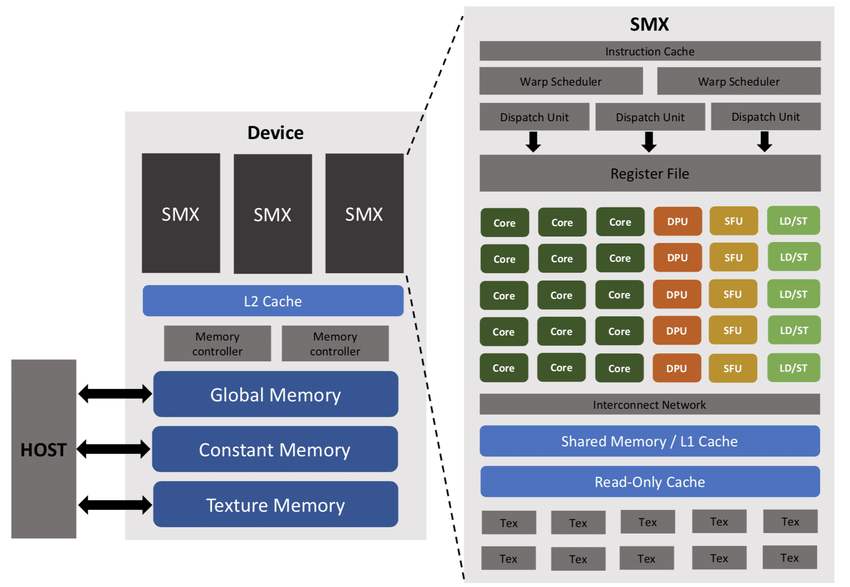
\includegraphics[width=\textwidth]{pictures/gpu_architecture.png}
            \caption{Архитектура GPU}
            \label{fig:architecture}
        \end{figure}
    \end{minipage}\hfill
    \begin{minipage}[m]{0.55\linewidth}
        \begin{itemize}
            \item Неграфические вычисления общего назначения на GPU
            \item Хорошо подходит, когда необходимо обрабатывать множество данных фиксированным набором команд
            \item Можно использовать для выполнения операций линейной алгебры над разреженными данными
        \end{itemize}
    \end{minipage}
\end{frame}

\begin{frame}[fragile] \frametitle{Cubool}
    \begin{center}
    \begin{minipage}[m]{0.85\linewidth}
        \begin{figure}
            \centering
            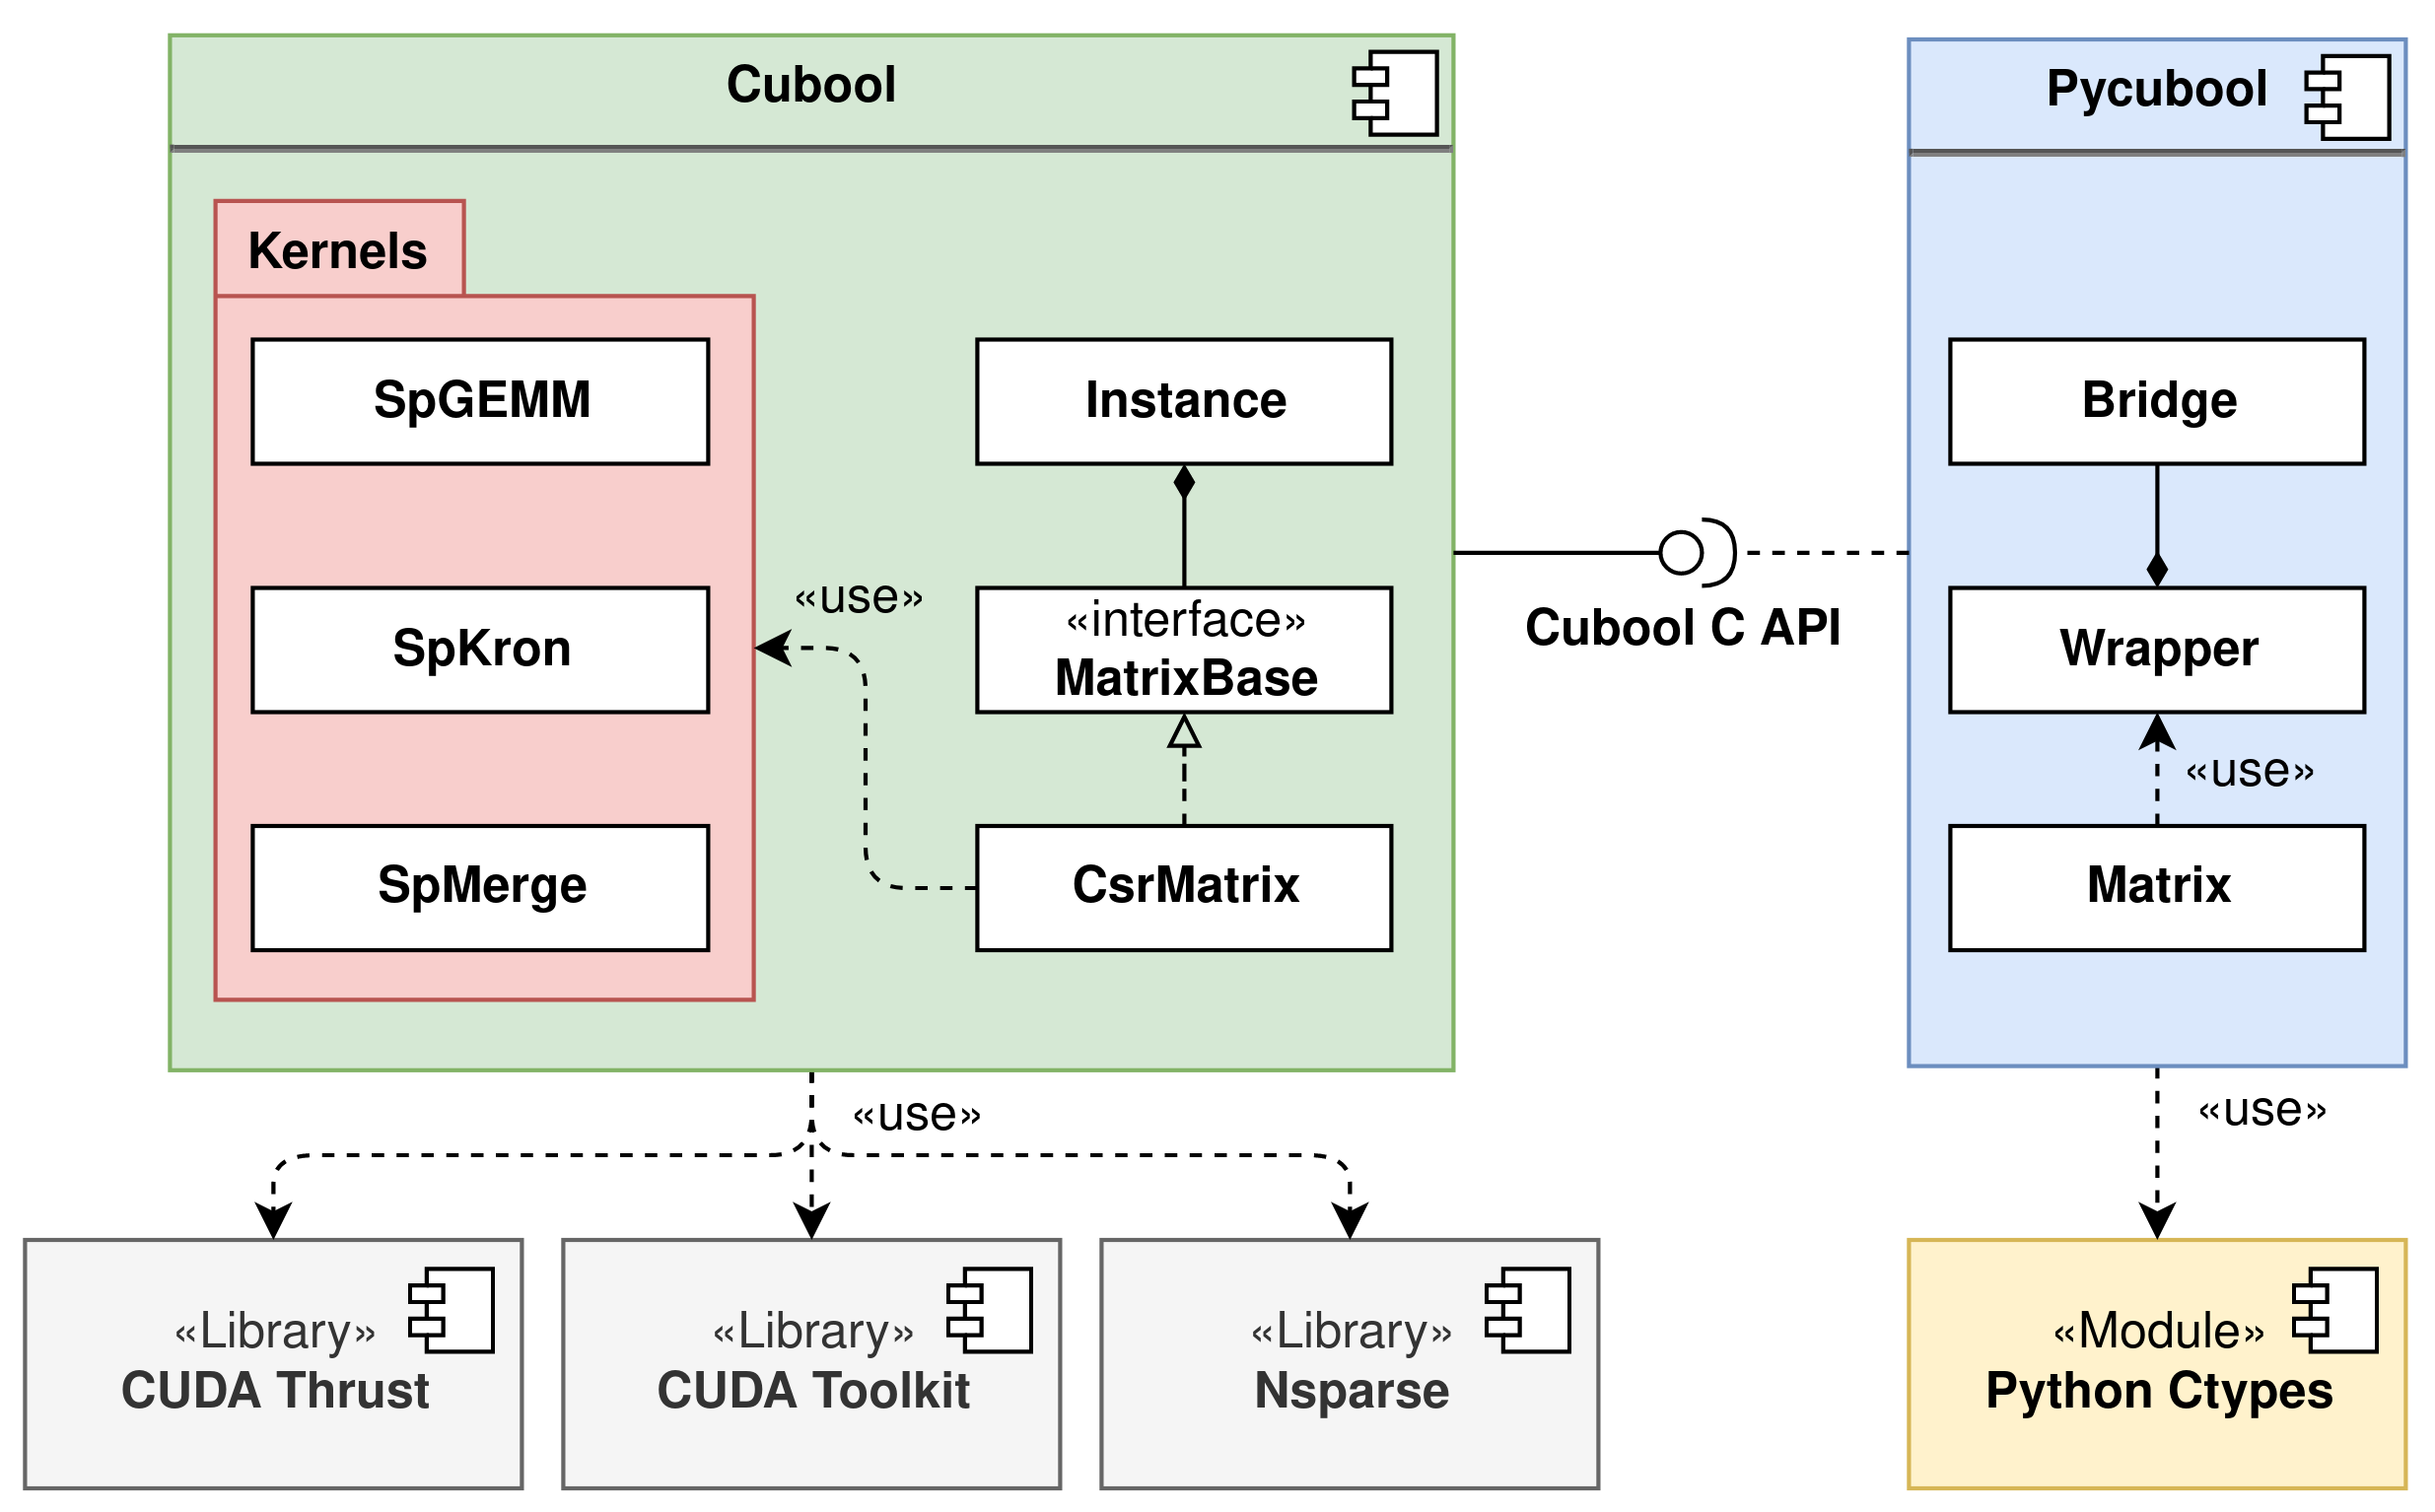
\includegraphics[width=\textwidth]{figures/lib_architecture.png}
            \caption{Архитектура библиотеки \textbf{Cubool}}
        \end{figure}
    \end{minipage}\hfill    
    \end{center}
\end{frame}

\begin{frame}[fragile] \frametitle{Пример использования C API}
    \begin{center} 
    \begin{minipage}[m]{0.85\linewidth}
        \begin{figure}
            \centering
            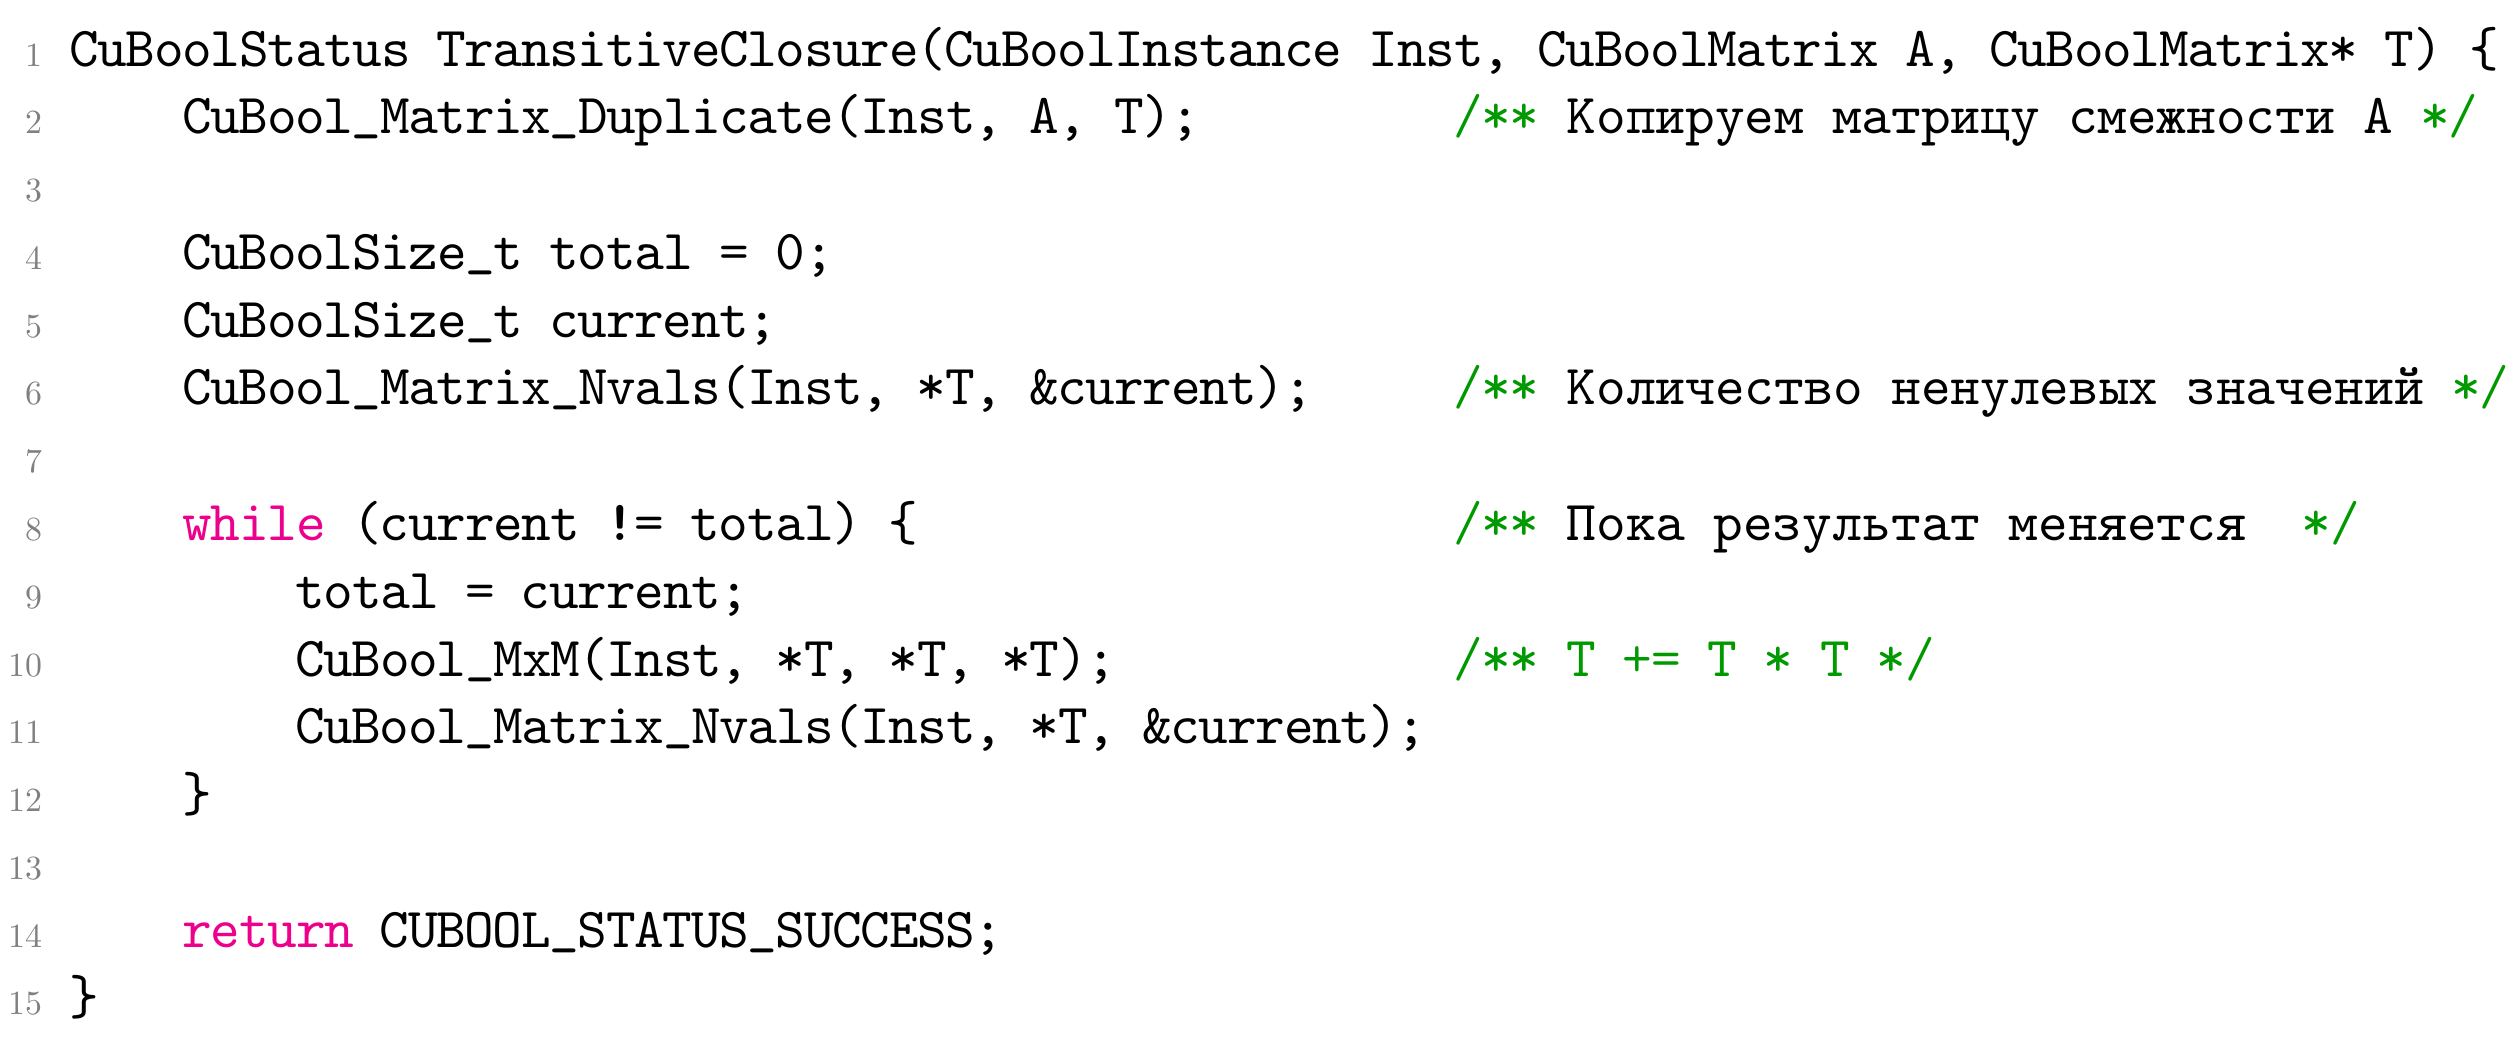
\includegraphics[width=\textwidth]{figures/tc_c_api.png}
            \caption{Вычисление транзитивного замыкания для ориентированного графа без меток с использованием \textbf{Cubool C API}}
        \end{figure}
    \end{minipage}\hfill    
    \end{center}   
\end{frame}

\begin{frame}[fragile] \frametitle{Пример использования Python API}
    \begin{center}
     \begin{minipage}[m]{0.85\linewidth}
        \begin{figure}
            \centering
            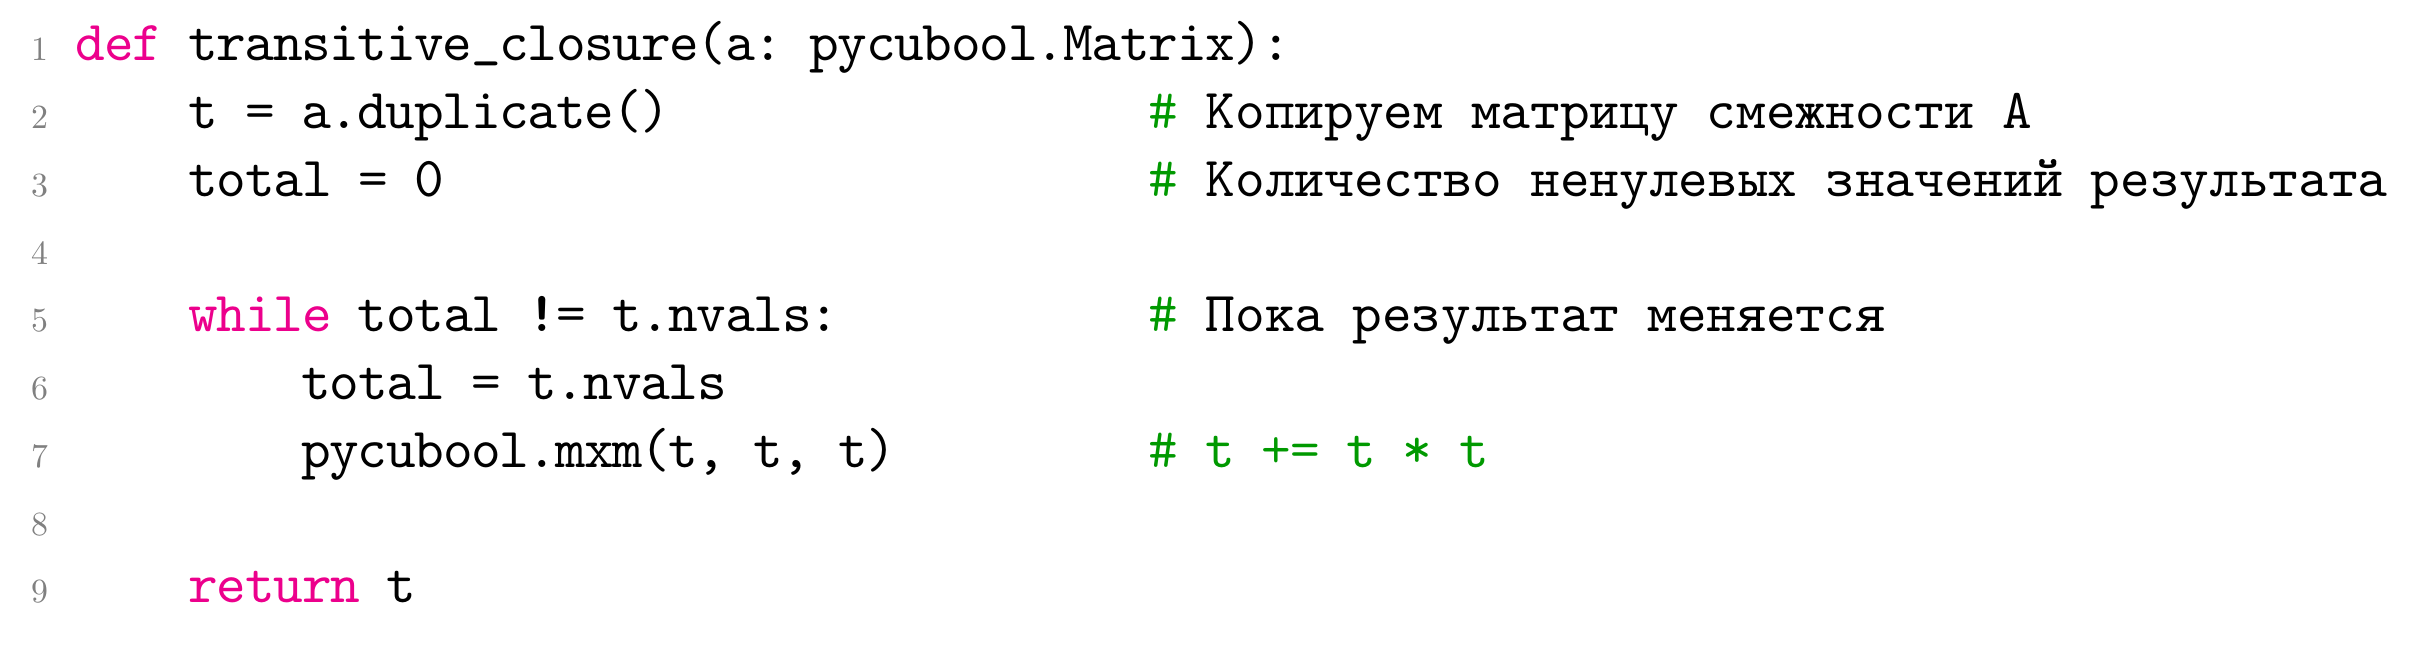
\includegraphics[width=\textwidth]{figures/tc_python_api.png}
            \caption{Вычисление транзитивного замыкания для ориентированного графа без меток с использованием \textbf{Pycubool}}
        \end{figure}
    \end{minipage}\hfill   
    \end{center}
\end{frame}

\begin{frame}[fragile] \frametitle{Задачи на ближайшее время}
    \begin{itemize}
        \item Реализация алгоритма поиска путей с КС ограничениями через произведение Кронекера с использованием примитивов библиотеки
        \item Экспериментальное исследование реализованного алгоритма
        \item Сравнение с реализацией на основе библиотеки  \textbf{GraphBlast}\footnote{https://github.com/gunrock/graphblast}
        \item Исследование возможности расширения библиотеки для выполнения операций в произвольном полукольце
    \end{itemize}
\end{frame}

% \begin{frame}[fragile] \frametitle{Пример графа и матрицы}
%     \begin{minipage}[m]{1.0\linewidth}
%         \begin{figure}
%             \centering
%             \begin{subfigure}[b]{0.47\textwidth}
%                 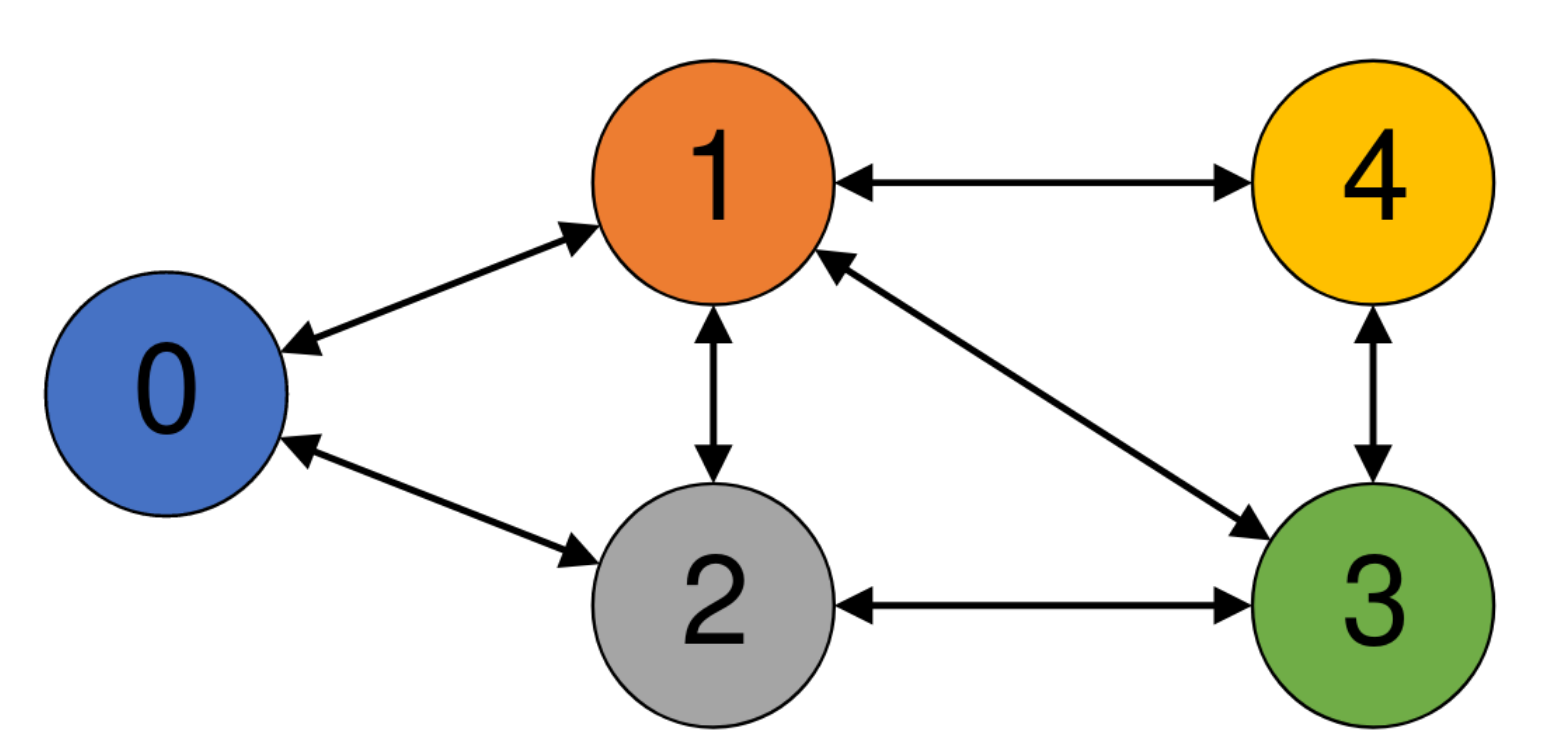
\includegraphics[width=\textwidth]{figures/graph.png}
%                 \caption{Graph}
%             \end{subfigure}
%             \hfill
%             \begin{subfigure}[b]{0.47\textwidth}
%                 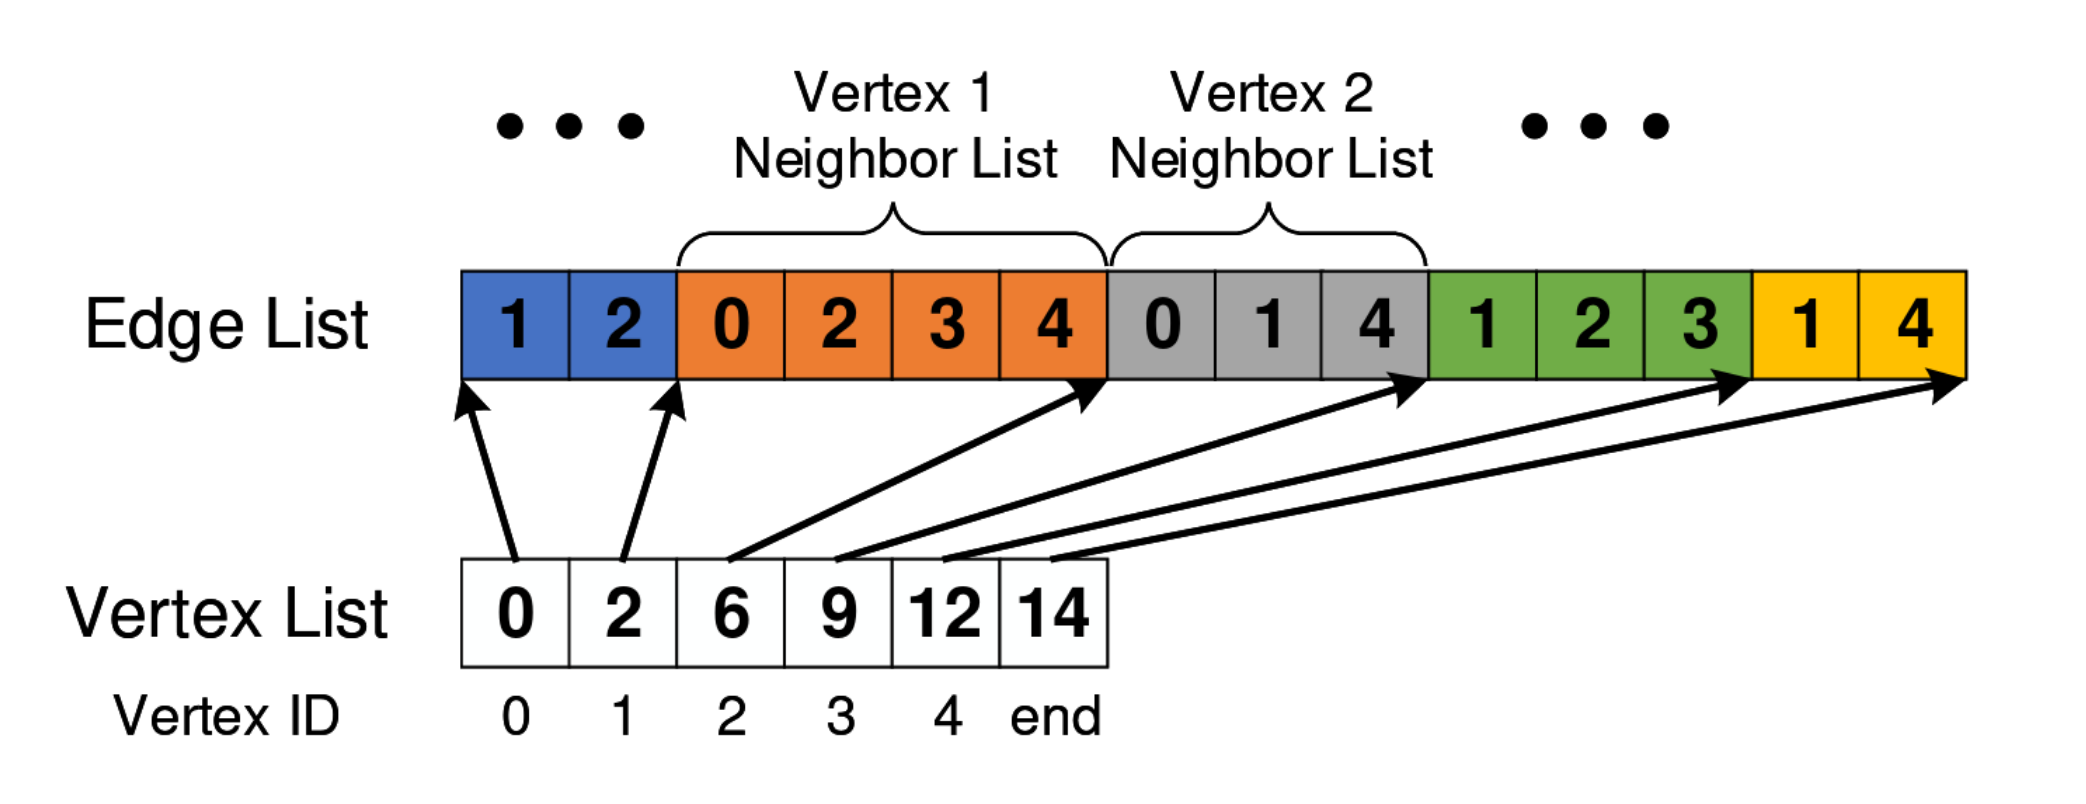
\includegraphics[width=\textwidth]{figures/csr_matrix.png}
%                 \caption{CSR matrix}
%             \end{subfigure}
%             \caption{Sample directed graph and its CSR adjacency matrix}
%         \end{figure}
%     \end{minipage}\hfill
% \end{frame}

% \begin{frame}[fragile] \frametitle{Результаты}
%     \begin{center}
%     \begin{minipage}[m]{0.85\linewidth}
%         \begin{figure}
%             \centering
%             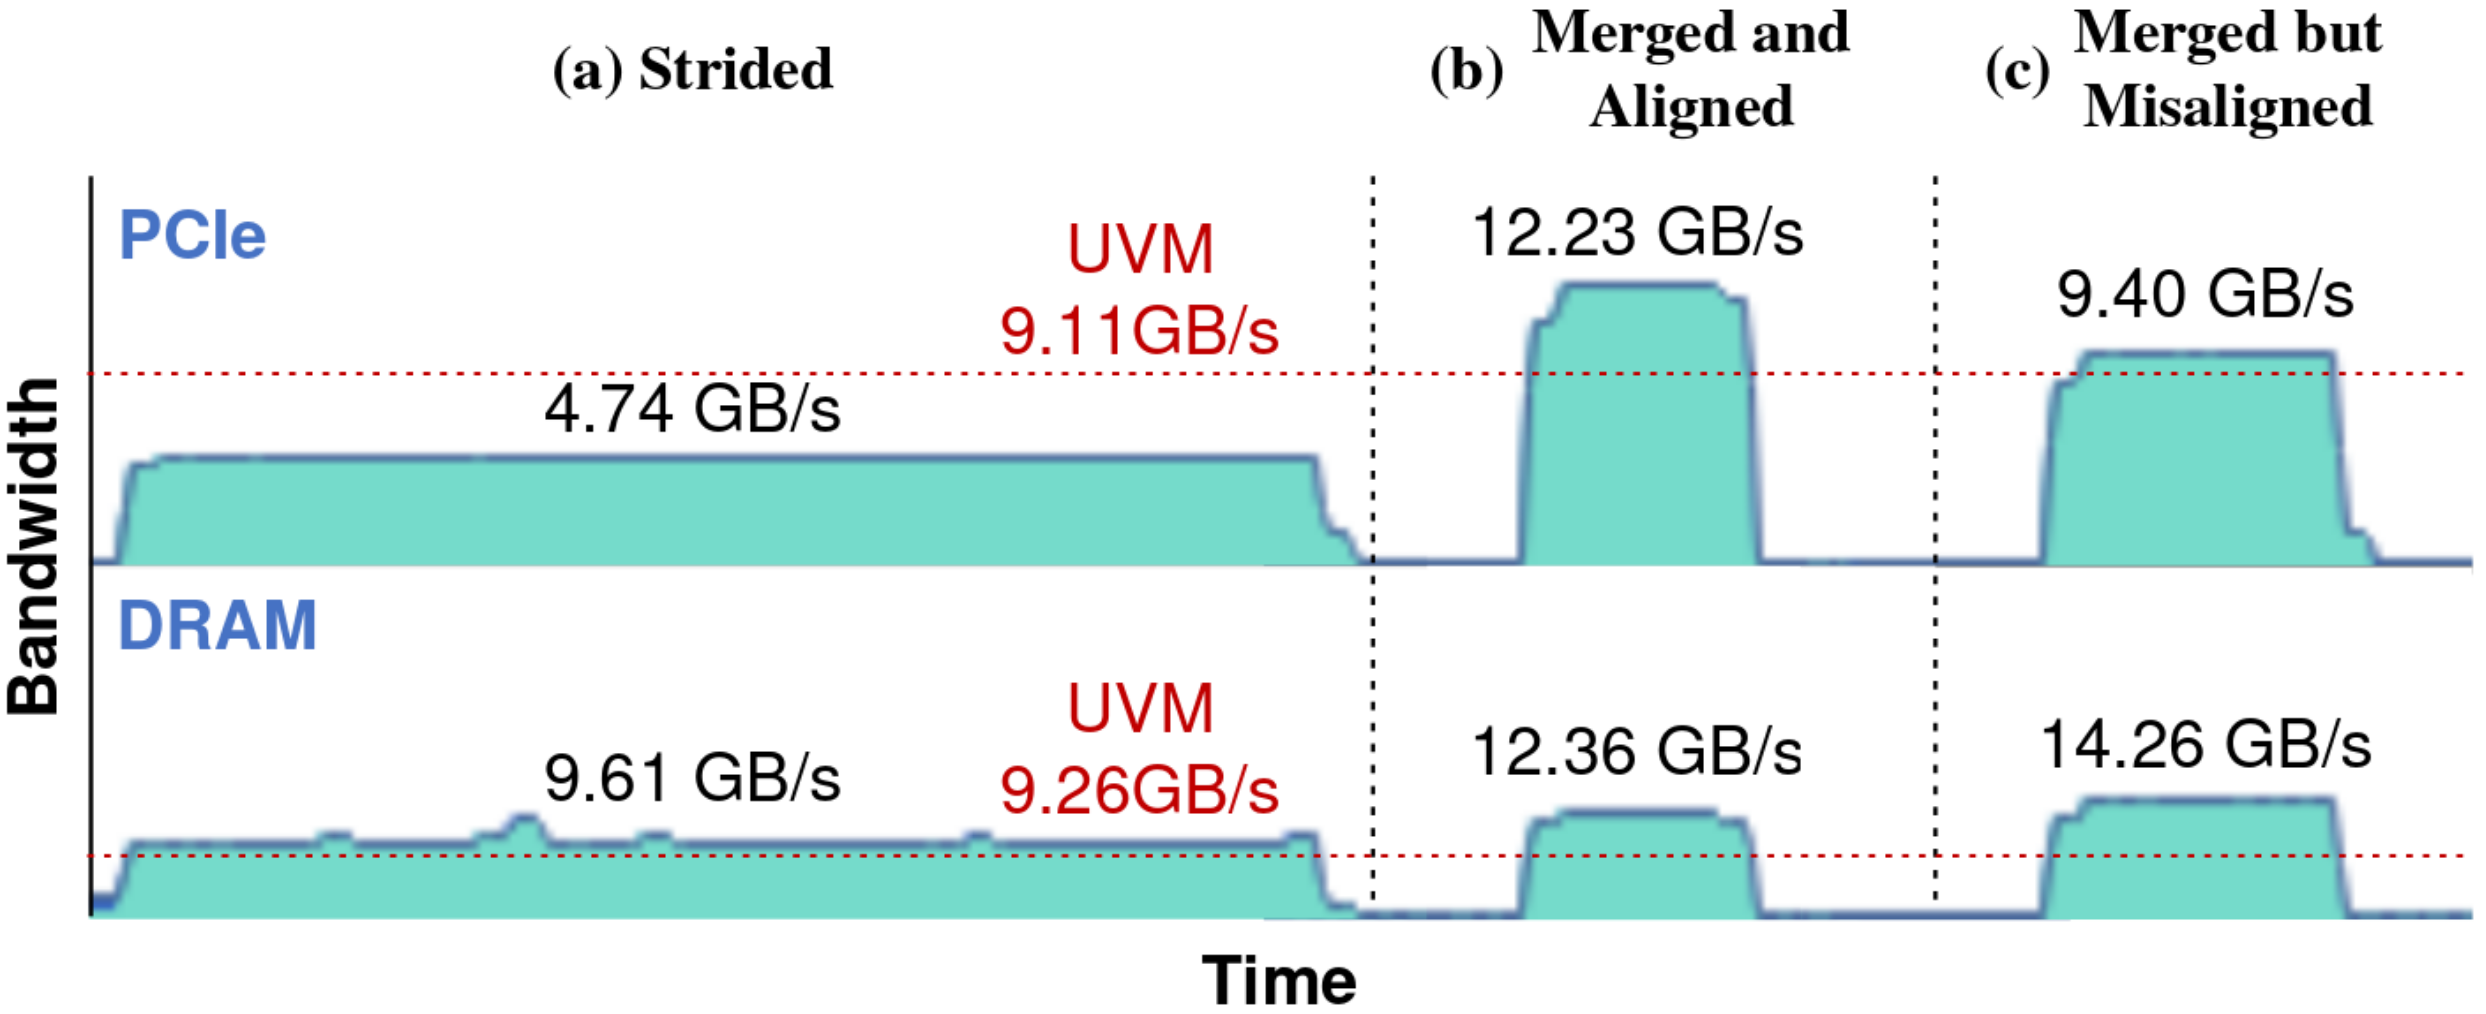
\includegraphics[width=\textwidth]{figures/access_patterns_utilization.png}
%             \caption{Average PCIe and DRAM bandwidth utilization for the dif-ferent zero-copy access patterns}
%             \label{fig:access_patterns_utilization}
%         \end{figure}
%     \end{minipage}\hfill
%     \end{center} 
% \end{frame}

% \begin{frame}[fragile] \frametitle{EMOGI}
%     \begin{minipage}[m]{1.0\linewidth}
%         \begin{figure}
%             \centering
%             \begin{subfigure}[b]{0.44\textwidth}
%                 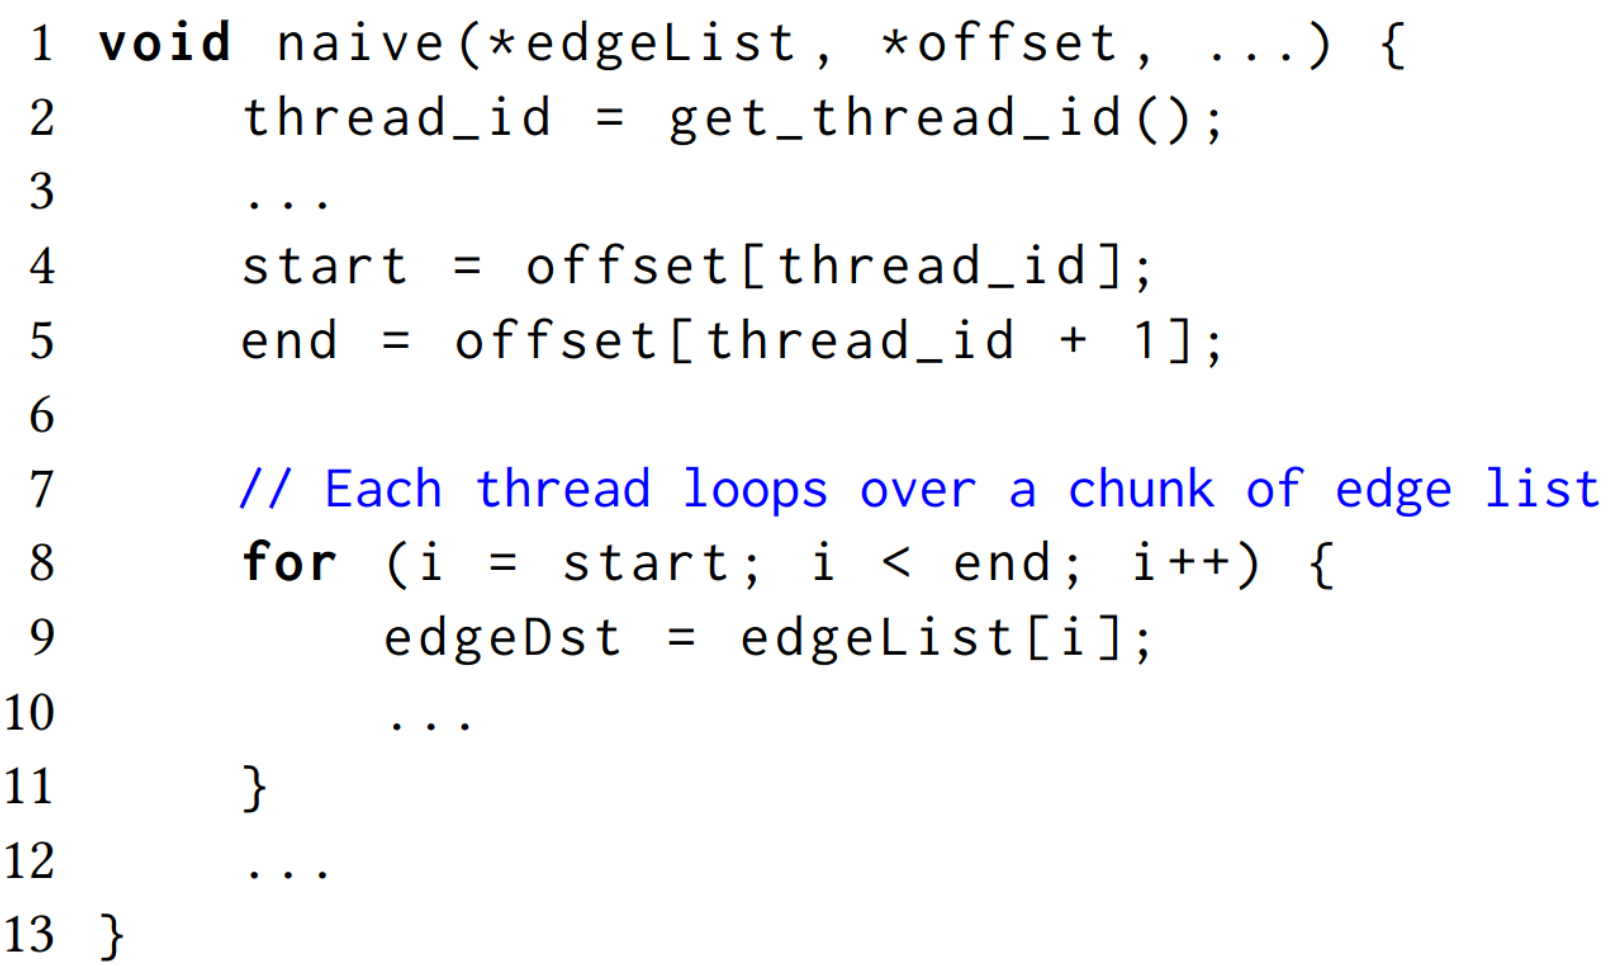
\includegraphics[width=\textwidth]{figures/emogi_naive.png}
%                 \caption{Na\"{\i}ve Uncoalesced Memory Access}
%             \end{subfigure}
%             \hfill
%             \begin{subfigure}[b]{0.44\textwidth}
%                 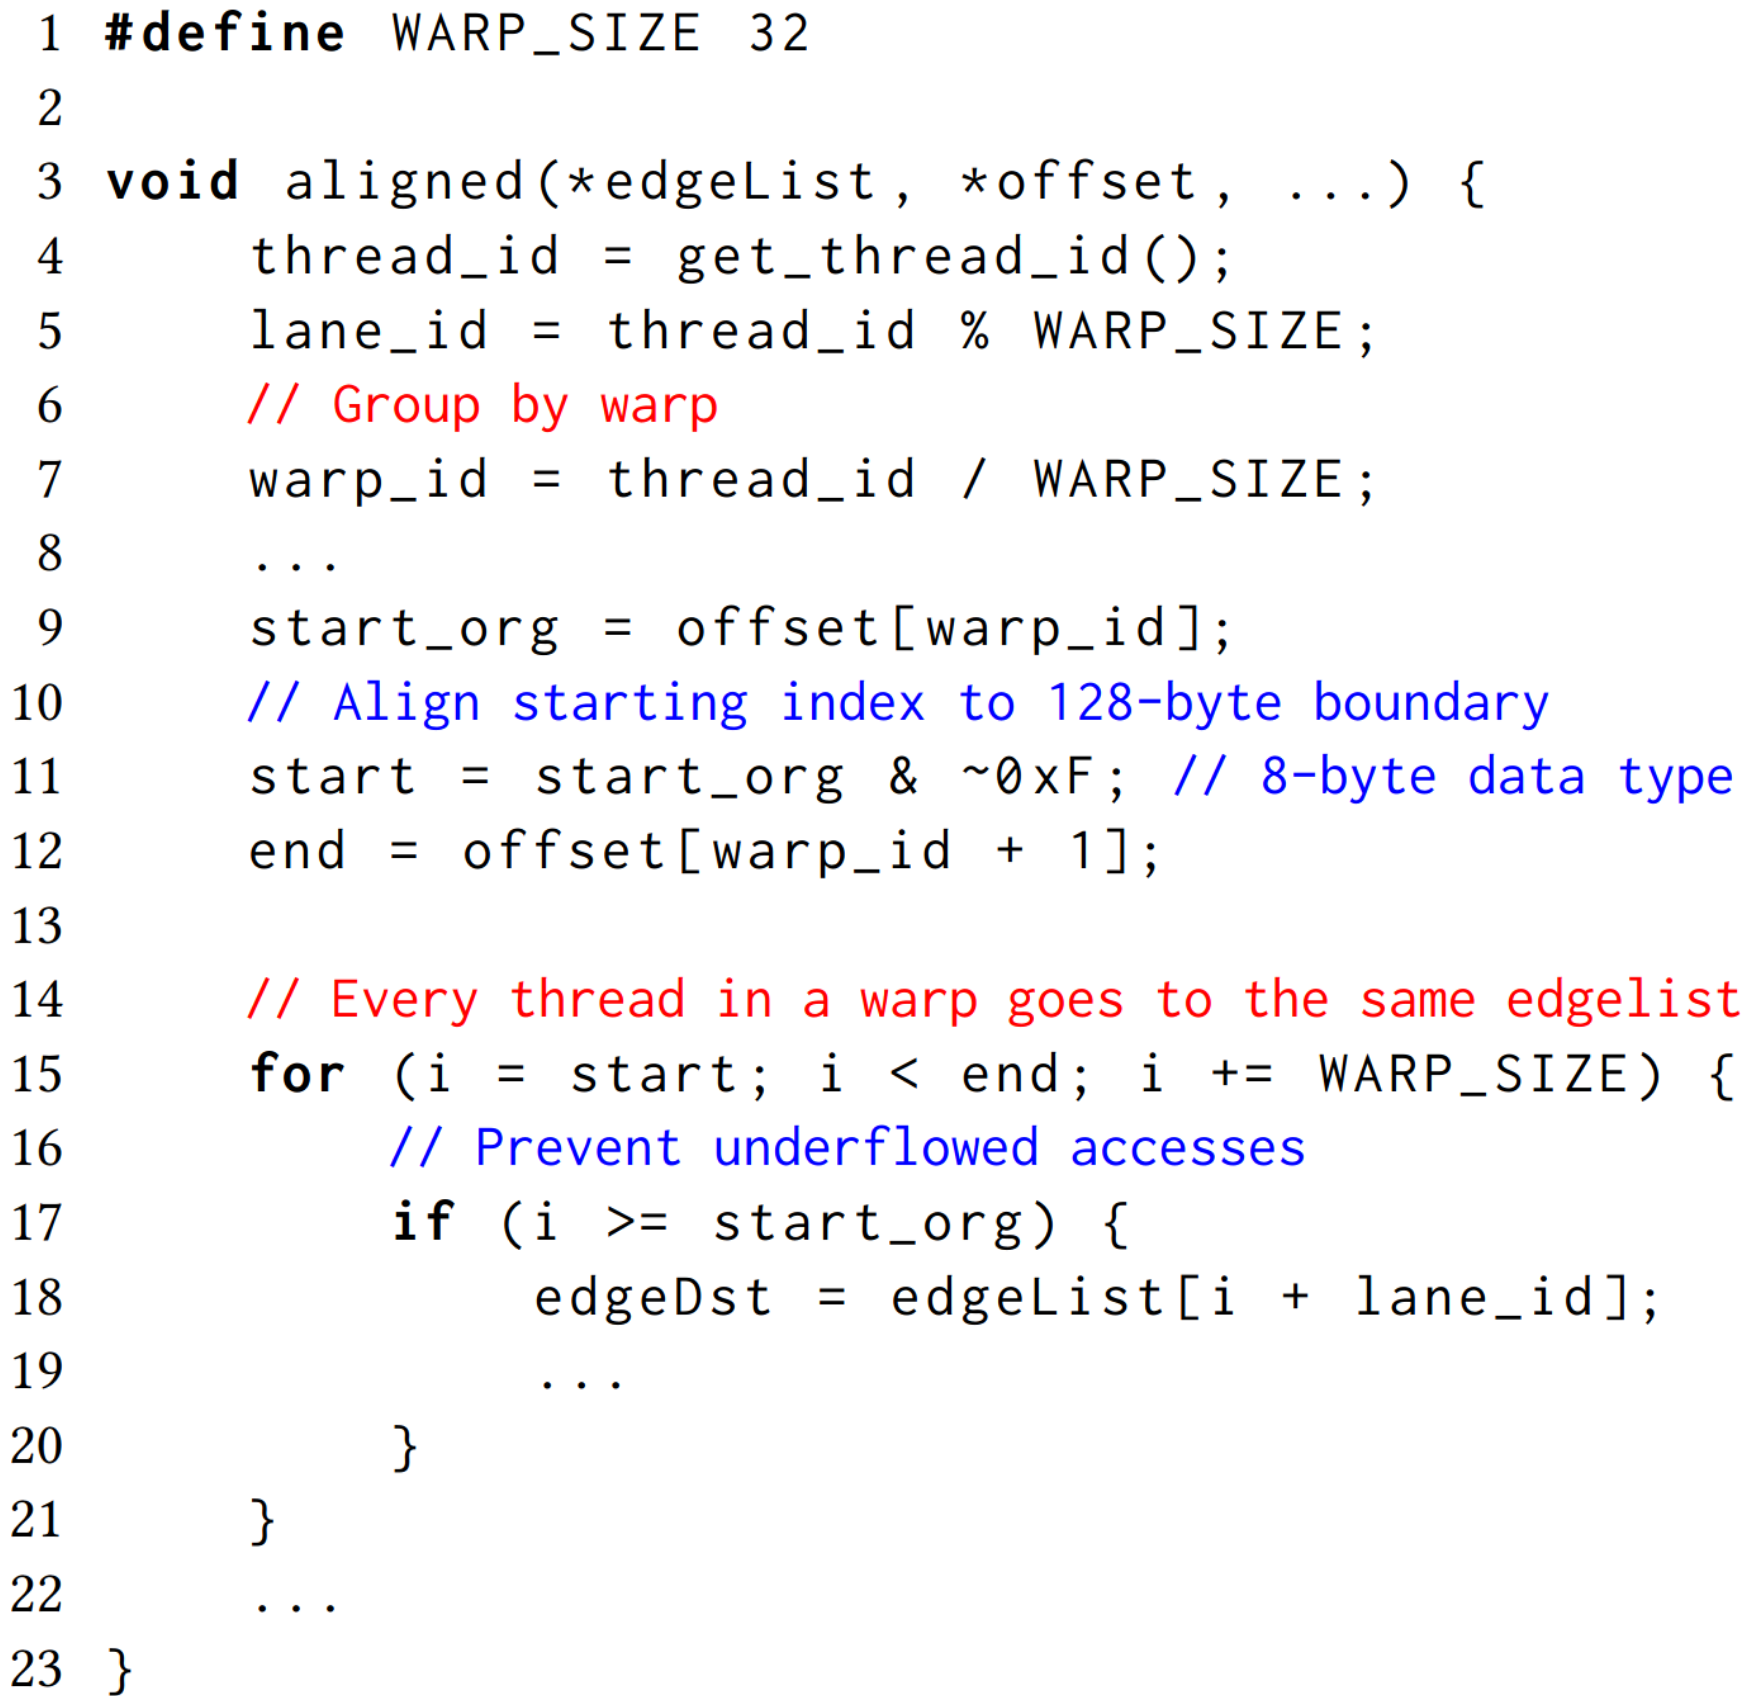
\includegraphics[width=\textwidth]{figures/emogi.png}
%                 \caption{EMOGI Coalesced Memory Access (Merged and Aligned)}
%             \end{subfigure}
%             \caption{Code listing for solution}
%         \end{figure}
%     \end{minipage}\hfill
% \end{frame}

\begin{frame} \frametitle{Дополнительно}
    \begin{itemize}
        \item Почта: \href{mailto:egororachyov@gmail.com}{egororachyov@gmail.com}
        \item Материалы презентации:
        {
            \begin{itemize}
                \item Arseniy Terekhov \& Artyom Khoroshev \& Rustam Azimov \& Semyon Grigorev (2020). Context-Free Path Querying with Single-Path Semantics by Matrix Multiplication. 1-12. 10.1145/3398682.3399163. 
                \item Egor Orachev \& Ilya Epelbaum \& Rustam Azimov \& Semyon Grigorev. (2020). Context-Free Path Querying by Kronecker Product. 10.1007/978-3-030-54832-2\_6. 
            \end{itemize}
        }
        \item Ссылка на проект Cubool: \href{https://github.com/JetBrains-Research/cuBool}{https://github.com/JetBrains-Research/cuBool}
    \end{itemize}
\end{frame}

\end{document}
